% SPDX-License-Identifier: LPPL-1.3c
% Copyright (C) 2026 Christophe Jorssen
% Author and Current Maintainer: Christophe Jorssen <christophe.jorssen@gmail.com>
% LPPL maintenance status: maintained
% This file is part of luafemm. See LICENSE and LICENSES.md for its terms.
\section{Axisymmetric electrostatic finite elements}
\label{sec:electric-axisymmetric}

The physical declarations in Section~\ref{sec:electric-fe} also describe
bodies of revolution. Use the following symmetry choice before declaring any
physical path. The guided examples in Section~\ref{sec:tutorial-electric-axisymmetric}
show spherical capacitors, circular plates, charged spheres and finite cylinders.

\begin{key}{/femm/electrostatic/problem type=\meta{planar or axisymmetric} (initially planar)}
Picture-local physical choice, for |model=finite elements| only.
|planar| uses translation perpendicular to the drawing. |axisymmetric| uses
revolution about $r=0$, with TikZ coordinates $(x,y)=(r,z)$ and $r\geq0$.
The computational domain remains rectangular in this half-plane. If |xmin|
is not explicitly assigned in the active TeX scope, its axisymmetric default
is zero; the planar default remains $-3$. A positive |xmin| describes an
annular computational region with an ordinary inner boundary. A negative
axisymmetric |xmin| is rejected. The other bounds retain their usual defaults.
A restored snapshot owns its problem type; attempting to change it fails.

Do not supply |depth| for an axisymmetric model, even with value one. Its
integrals already cover the full $2\pi$ revolution. Display scale, rotation,
colours and line styles change no physical length or axis definition.
\end{key}

\begin{codeexample}[width=0pt]
\begin{tikzpicture}[femm/electrostatic={model=finite elements,
    problem type=axisymmetric,xmax=1,ymin=0,ymax=1,
    outer boundary=insulated,mesh size=.25,name=axial reference}]
  \draw[thick,femm/electric electrode={name=bottom,potential=10}]
    (0,0)--(1,0);
  \draw[thick,femm/electric electrode={name=top,potential=0}]
    (0,1)--(1,1);
  \pic {femm electric field};
  \pic[femm/electric={levels={2,4,6,8}}] {femm equipotentials};
  \draw[densely dashed,gray] (0,0)--(0,1);
  \path[femm/electric profile={name=axial reference profile,samples=21}]
    (.5,0)--(.5,1);
\end{tikzpicture}
\end{codeexample}

This example has an insulating cylindrical side wall, so it tests a uniform
axial field without fringing. The axis is a regularity boundary, not a grounded
wire. Its dielectric potential may vary with $z$. Only an |insulated| boundary
path may be placed wholly on the axis; an explicit voltage or normal
 displacement there fails. Electrode and charged-layer closure segments lying
on the axis have zero area and contribute no surface condition. An entirely
axis-only electrode or charged path is rejected. A solid conductor still fixes
all its interior nodes, including axial ones. Endpoints belonging to a
nonzero-area electrode surface retain that electrode's voltage.

\subsection{Components, coordinates and full-body integrals}
\begin{key}{/femm/electric plot/component=\meta{V, E, Er, Ez, D, Dr, Dz, Ex, Ey, Dx or Dy} (initially E)}
The additional choices |Er|, |Ez|, |Dr| and |Dz| require a profile captured
from an axisymmetric FE model. They alias |Ex|, |Ey|, |Dx| and |Dy| in its
meridional coordinate frame. The Cartesian spellings remain accepted.
Fields use V/m and displacements C/m$^2$. There is no azimuthal component
for this scalar, axisymmetric electrostatic problem. The aliases are rejected
for planar FE and analytical models to prevent an ambiguous interpretation.
One-sided limits and NaN gaps at element/material interfaces are preserved.
\end{key}
\begin{key}{/femm/electric plot/abscissa=\meta{s, x, y, t, r or z} (initially s)}
|r| and |z| require an axisymmetric FE profile and alias the model-coordinate
|x| and |y| abscissas. They use the model length unit, not metres unless
|length unit=m|. The default |s| remains arclength along the captured contour.
\end{key}
\begin{key}{/femm/electric value/quantity=\meta{quantity} (initially charge)}
For axisymmetric FE, |charge| returns total source charge in C without an
|electrode| selector, or that electrode's variational reaction charge with one.
|energy| returns the full-body field energy in J. The |outer boundary| selector
still collects the reactions on prescribed exterior voltages.
|charge per length|, |energy per length| and |charge balance per length| are
unavailable in this geometry; asking for one fails explicitly.
|nodes|, |triangles|, |iterations| and |relative residual| retain their FE meanings.
\end{key}
\begin{key}{/femm/electric value/quantity/charge balance}
Global signed residual, in C, of total volume/sheet source charge plus all
prescribed-voltage reactions minus the prescribed outward displacement flux.
This choice is available for both FE geometries; planar results include |depth|.
It is a conservation diagnostic, not an error estimate for the field.
Do not combine it with an |electrode| selector.
\end{key}

\begin{codeexample}[width=0pt]
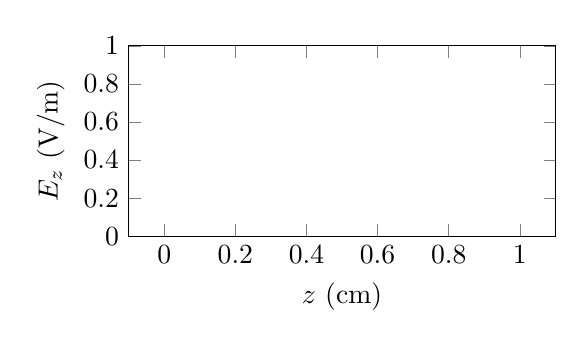
\begin{tikzpicture}
\begin{axis}[width=7cm,height=4cm,no markers,
    xlabel={$z$ (cm)},ylabel={$E_z$ (V/m)},ymin=900,ymax=1100]
  \femmelectricplot[profile=axial reference profile,component=Ez,abscissa=z]
\end{axis}
\end{tikzpicture}
\quad
$Q=\femmelectricvalue[model=axial reference,electrode=bottom,quantity=charge]
  \,\mathrm C$.
\end{codeexample}

\subsection{Weighted formulation and numerical interpretation}
For a meridional dielectric domain $\Omega$, $\mathbf E=-\nabla V$ and
$\mathbf D=\epsilon\mathbf E$. The weak equation is
\[
 \int_\Omega 2\pi r\,\epsilon\,\nabla V\cdot\nabla w\,dr\,dz
 =\int_\Omega 2\pi r\,\rho w\,dr\,dz
 +\int_{\Gamma_\sigma}2\pi r\,\sigma w\,ds
 -\int_{\Gamma_g}2\pi r\,g w\,ds,
 \qquad g=\mathbf D\cdot\mathbf n.
\]
It is a scalar Poisson operator. It does not reuse the magnetic
azimuthal-vector-potential operator or its axis constraint.
On each affine triangle, $r$ is linear and the shape gradients are constant;
the stiffness weight is the exact centroid radius. The volume source uses
the exact $\int_T rN_i$, and edge loads use the exact $\int_e rN_i$.
This differs from equally distributing a centroid-weighted source among nodes.
The rectangular mesh, its constrained curved-path approximation and the
isotropic constitutive restrictions are otherwise the same as in planar FE.

Energy integrates $\tfrac12\mathbf E\cdot\mathbf D$ with the same volume
weight. Charges are full-system reactions before voltage elimination, so
energy, sources and boundary fluxes use one consistent discretization.
Positive surface density adds outward displacement jump; positive prescribed
exterior displacement leaves the domain. The regular axis has zero surface
measure and needs no pointwise $1/r$ expression during assembly.

The raw P1 gradient is constant on a triangle. On a coarse mesh its radial
component need not vanish pointwise on the axis, even though the weak solution
approaches the regular solution under refinement. No cosmetic clamp or hidden
field recovery is applied. Field lines stop at the half-plane boundary;
negative radii are not another physical domain. Curved electrode faceting,
mesh resolution and an artificial exterior boundary require separate
sensitivity checks. General three-dimensional objects, azimuthally varying
charges and singular axial line charges are not implemented by this scalar
FE provider. Floating conductors and supported meridional dielectric tensors
are described in Section~\ref{sec:electric-extended}.
